\section{Evaluation}
\label{sec:eval}
We systematically evaluate \sys on four bulk-semantic processing applications from the AI and data literature:  fact-checking, biomedical multi-label classification, search, and topic analysis. 
Some of these applications can be expressed by recent LLM-based analytics systems, like AI UDFs, UQE and DocETL, allowing us to compare against them; while other applications are not supported by the baseline systems, but LOTUS supports them. For each application, we additionally compare against strong hand-designed pipelines from the literature. We evaluate the LOTUS optimizer, comparing the performance of optimizations for semantic filters, joins, top-k and group-by with our gold algorithms. Lastly, we analyze the statistical accuracy guarantees provided by LOTUS' optimizations. Overall, we find the following:
\begin{itemize}
    \item Compared to AI-based analytics systems, like AI UDFs, UQE, and DocETL, LOTUS attains similar or up to $170\%$ higher accuracy, while running up to $3.6\times$ faster and offering statistical accuracy guarantees that the other systems do not provide.
    \item Compared to hand-written pipelines from the AI literature for fact-checking, biomedical classification, and search, LOTUS matches state-of-the-art quality, or exceeds it by up to $100\%$, in programs involving a few semantic operators.
    \item The LOTUS optimizer can substantially reduce cost of semantic operator programs, by up to $1,000\times$ compared to high-quality gold algorithms, and provides accuracy guarantees, which hold across repeated trials.
\end{itemize}

To report controlled latency numbers, we run each baseline and experiment locally on 4 80GB A100 GPUs using Llama-3-70B~\cite{noauthor_introducing_nodate} and E5 embeddings~\cite{wang_text_2024}, with a batch size of 64 running on vLLM~\cite{kwon_efficient_2023}, unless otherwise stated. To run DocETL baselines and reproduce some of their benchmarks~\cite{shankar_docetl_2024}, we additionally use OpenAI~\cite{noauthor_openai_nodate} models, including GPT-4o-mini-2024-07-18, GPT-4o-2024-08-06 model, and text-embedding-3-small, where noted. For our experiments that use OpenAI models , we control for cost by limiting execution to 64-way thread parallelism. For reproducibility, we set temperature to $t=0$ for all methods and baselines, unless otherwise stated.

\subsubsection{Benchmarked Methods}
We briefly overview the main methods we benchmark and tested parameters.

\heading{AI UDFs.} Many database vendors~\cite{vertexai,  databricks, noauthor_large_nodate, motherduck_introducing_nodate, williamdassafmsft_intelligent_2024, noauthor_snow_nodate} now support AI UDFs, which include map-like, row-wise LLM operations and primitives for vector search. To control for serving infrastructure, we implement these programs using LOTUS running on vLLM, and restrict our API to \verb|sem_map|, \verb|sem_search| and \verb|sem_sim_join|.

\heading{UQE.} UQE~\cite{dai_uqe_2024} proposes an optimized LLM-powered filter method, which is relevant to this work. UQE also optimizes non-LLM aggregates (e.g. COUNT) integrated with LLM-based queries, but this is beyond the scope of our evaluation. Since the code is not open-source, we implement the UQE filter in about 100 line of code in python. The UQE filter method takes an LLM call budget and provides a best-effort embedding-based approximation. In contrast, LOTUS provides a general proxy-oracle approximation method, where the proxy may be embedding-based or LLM-based. To provide a fair comparison between UQE and LOTUS, we normalize the \emph{latency budget} when comparing against LOTUS programs that use LLM-based proxies, and we normalize \emph{the LLM call budget} when comparing against LOTUS programs that use embedding-based proxies. We also hyper-parameter tune the mini-batch size used for UQE's active learning algorithm. 

\heading{DocETL.} DocETL~\cite{shankar_docetl_2024} uses an LLM agent as the query optimizer to perform rewrites to programs, allowing programs to specify separate LLMs for the optimizer and execution. Our experiments find that the optimizer often fails, and among runs where the optimizer succeeds, performance varies. Based on personal communication with the authors, we run the DocETL baselines multiple times. We obtain three successful runs and report the average performance of these three successes.
We also try using both Llama-70B as the DocETL optimizer, following our setup for each other baseline, and GPT-4o-mini as the DocETL optimizer, following the DocETL preprint~\cite{shankar_docetl_2024}. However, we find both fail to produce a successful run in Section~\ref{subsec:biodex}.
After reaching out to the authors, we confirm a mistake in the pre-print and find that GPT-4o is required for the DocETL optimizer for our evaluation on BioDEX in Section~\ref{subsec:biodex}.
We also note we found several bugs in the DocETL codebase, which we have done our best to fix and have also coordinated with the authors about. Since the codebase is an evolving artifact, we report the commit number we used for our evaluation\footnote{\url{https://github.com/ucbepic/docetl/commit/93050998077a9eb6fc1ee99dc96d1e0a222a987f}}.


\heading{LOTUS.} We set default accuracy targets of $\gamma=0.9$ and failure probabilities of $\delta=0.2$. We provide a detailed ablation, varying these parameters in Section~\ref{subsec:ablation}. Additionally, our sampling size uses $0.01\%$ of the data, similar to other works~\cite{shankar_docetl_2024}, and a minimum sample size of $s=100$ for smaller datasets, following prior work~\cite{kang_approximate_2020}.


\subsection{Fact-Checking}
\label{subsec:factchecking}
Fact-checking systems determine whether a given claim is correct, typically based on verifiability with a knowledge corpus. 
FacTool~\cite{chern_factool_2023} is a recent open-source research work that provides a  multi-step fact-checking pipeline, involving claim extraction, query generation, tool querying, evidence collection, and verification. We consider the task of using constructing the FacTool pipeline, which was originally written in over 750 lines of code. We use the FEVER \cite{thorne_fever_2018} dataset, a claim verification dataset, for our evaluation. Claim verification is based on a corpus of $~5.5$ million Wikipedia articles, and each claim is labeled with one of three gold labels, "Supported", "Refuted", or "NotEnoughInfo". We merge the latter two labels into a single class, "Not Supported", following prior work~\cite{chern_factool_2023} for our evaluation. To control for our API spending budget, we sample 1,000 claims from the development dataset. 

\heading{Baselines.} 
For all baselines we use ColBERT~\cite{khattab_colbert_2020} as the retreiver model\footnote{FactTool's pipeline, by default, performs retrieval with a Google Search API \cite{noauthor_custom_nodate}. We evaluate the pipeline with both the default retrieval API, and with the open-source ColBERT \cite{khattab_colbert_2020} index. We find that the results are similar, and we report the results using ColBERT for retrieval to hold the retriever model constant with the other baselines.} and Llama-70B served with vLLM. We run FactTool's open source codebase~\cite{noauthor_gair-nlpfactool_nodate} to measure its performance.
The AI UDF baseline uses a simple semantic map-search-map dataflow, following FacTool's pipeline. First each claim is mapped to two search queries. Then the generated queries are used for search over the Wikipedia corpus. Lastly, each claim appended with retrieved context is mapped to truth label, along with a reasoning. We use the same prompts found in FacTool \cite{noauthor_gair-nlpfactool_nodate}, which include 3 demonstrations for generating search queries in the first semantic mapping, and chain-of-thought prompting in the second semantic mapping. The UQE baseline follows the first two steps of the AI UDF baseline, but replaces the final step with UQE's embedding-based LLM-powered filter. Our LOTUS program similarly follows a map-search-filter pipeline and uses a Llama-8B proxy model. To provide a fair comparison, we tune the UQE LLM call budget to normalize execution time with the optimized LOTUS program. Since DocETL does not provide search primitives, we are unable to benchmark it in this application.



\begin{footnotesize}
    
\begin{table}[!t]

\centering
\caption{\small Fact-checking Performance on the FEVER Dataset.}
\vspace{-.3cm}
\begin{threeparttable}
% \begin{tabular}{ccccc}
\begin{tabular}{p{2.2cm}p{1.cm}p{1.3cm}p{1.6cm}p{.6cm}}
% \hline
\toprule
Method & Accuracy & ET (s), with batching & ET (s), no batching & LoC\\
% \hline
\midrule
FacTool & 80.9 & N/A & 5396.11 & > 750\\
AI UDF: map, search, map & 89.9 & 688.9 & 4,454.2  & < 50\\
AI UDF map, search + UQE filter & 66.0 & 184.4 & 738.3 &  150\\
\sys map, search, filter (unopt.) & 91.2 & 329.1 & 989.0 & < 50\\
\sys map, search, filter (opt.)  & 91.0 & 190.0 & 776.37 & < 50\\
% \hline
% \sys-fact-join\liana{remove} & 84.5  & 11,951.35 & 60,364.39 & < 50\\
\bottomrule
\vspace{-.3cm}
\end{tabular}
% \begin{tablenotes}
% \centering
% \footnotesize
% % \item[*] $\gamma_R=\gamma_P=.9, \delta=0.2$ 
% \end{tablenotes}
\end{threeparttable}
\label{tab:factchecking}
\vspace{-.3cm}
\end{table}
\end{footnotesize}



\heading{Results.} We report the accuracy of each method, an estimate of lines of code (LoC), and average execution time over 10 runs in seconds, both with and without batching to provide a fair comparison with FacTool, which provides a sequential implementation only. 
Overall, Table~\ref{tab:factchecking} demonstrates that the optimized LOTUS program reproduces state-of-the art accuracy, comparable to that of FacTool, with $7\times$ faster unbatched execution and $28\times$ faster batched execution, and in less than 50 lines of user code, while also outperforming each baseline. 

Comparing the optimized LOTUS program to the AI UDF baseline, we see that both acheive comparable accuracy in relatively few lines of code. However, the LOTUS \verb|sem_filter| can be more heavily optimized compared to the generic AI UDF map operation. This allows the LOTUS program to attain $3.6\times$ faster execution, attributable to the \verb|sem_filter|'s short LLM generations, which leads to cheaper decoding, and our proxy-based optimization for filters. We also observe that the LOTUS program outperforms the UQE program by $38\%$ accuracy at an equivalent latency budget. While our filter optimization adaptively learns when to leverage the proxy in order to meet an accuracy target, UQE's embedding-based approximation provides no accuracy guarantees. 

Finally, we compare the optimized LOTUS program to the un-optimized LOTUS program. We observe that the optimized \sys program achieves $99.8\%$ accuracy relative to the un-optimized one, while reducing batched execution time by $1.7\times$. Figure~\ref{fig:factchecking_cascades} highlights the diverse performance trade-offs achievable by our \verb|sem_filter| approximation. The plot shows the accuracy and execution time of the LOTUS program using the gold algorithm with Llama 70B, or using the proxy only, shown respectively by the green and red circles.
By varying the filter recall and precision target, our cascade-based approximation offers diverse trade-offs between accuracy and execution time, shown by the stars.



\begin{figure}[t]
  \centering
  % \vspace{-.4cm}
  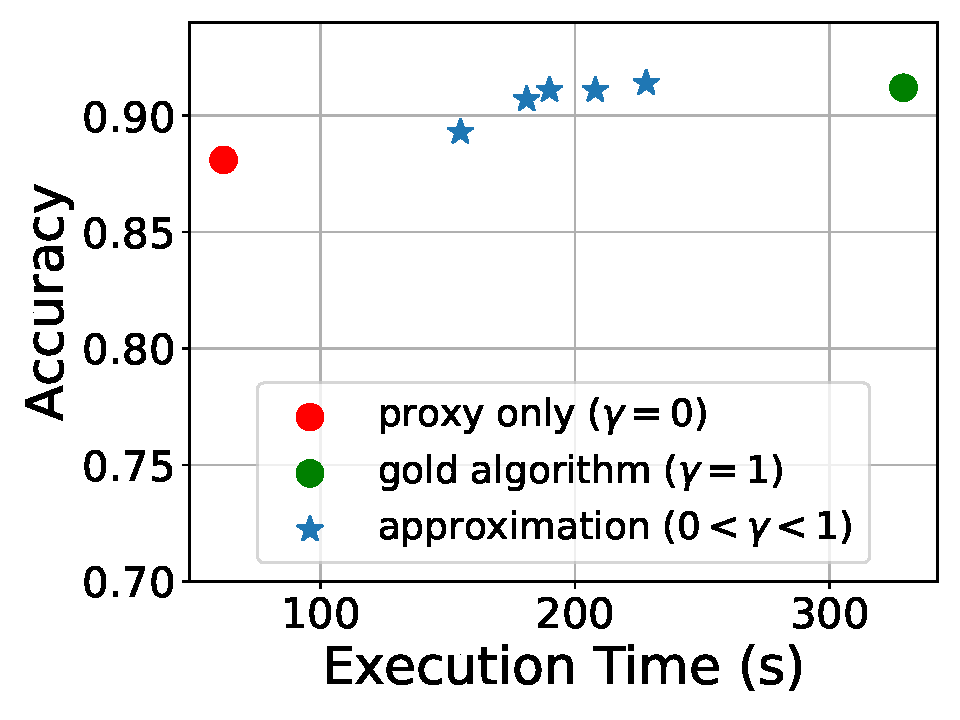
\includegraphics[width=.45\linewidth]{figures/factchecking_cascades.pdf}
  \vspace{-.5cm}
  \caption{\small Accuracy vs. execution time (s) for the \sys fact-checking program on the FEVER dataset. We compare the performance using the proxy only (red circle) or oracle only (green circle) for filters to the pipeline implemented using our filter approximation with both models for varied the precision and recall target, at $\delta=0.2$ (stars).}
  \label{fig:factchecking_cascades}
   \vspace{-.3cm}
\end{figure}



\subsection{Biomedical Multi-label Classification}
\label{subsec:biodex}


Biomedical classification entails processing complex, lengthy patient documents. We consider the extreme multi-label classification task on the BioDEX Dataset~\cite{doosterlinck_biodex_2023}, which consists of a corpus of $65,000$ biomedical articles, and ground-truth expert-created drug safety reports constructed from each article. The task is to classify the patient's drug reactions, given each medical article.  Notably, there are $~24,000$ possible drug-reaction labels, making this task an extreme multi-label classification task. Due to the large number of possible labels, leveraging an LLM to perform inference is difficult, and this setting has been studied in prior works~\cite{doosterlinck_-context_2024}. We show below that this task can be efficiently modeled and optimized using the semantic join. Similar to prior work~\cite{doosterlinck_biodex_2023} we sample 250 patient articles for our evaluation to control for our API spending budget.

\heading{Baselines.} 
The search baseline performs batched similarity search over each patient article and the set of reaction labels. For the baseline LLM-based analytics systems, we implement a LLM-powered join over the patient articles and set of candidate reaction labels, followed by a ranking step, if supported. The AI UDF program entails a naive, nested-loop join pattern using row-wise LLM operators; however we note this is prohibitively costly and we report estimated latency. While UQE does not explicitly study joins, we implement a UQE join using its optimized filter. The DocETL program uses a join and reduce, which uses listwise ranking, following the preprint~\cite{shankar_docetl_2024}. We note that we are unable to successfully run DocETL using Llama-70B or GPT-4o-mini for its optimizer so results (Table~\ref{tab:biodex}, \ref{tab:biodex_docetl}) are shown using GPT-4o for the DocETL optimizer. LOTUS supports both join and ranking. Although LOTUS provides a \verb|sem_topk| operator, we limit our ranking step to list-wise ranking to maintain a fair comparison with DocETL, and revisit ranking in Section~\ref{subsec:search}. 
Our main results are shown in Table~\ref{tab:biodex}, using Llama-70B and E5 embeddings and sampling size of $0.01\%$.
We also provide an additional set of benchmarks in Table~\ref{tab:biodex_docetl} comparing LOTUS and DocETL following the models, prompts and parameters used in the original DocETL preprint. The DocETL setup uses GPT-4o-mini, text-embedding-3-small embeddings and a sampling size of 500. Once again, DocETL fails when we attempt to use GPT-4o-mini for the optimizer, so we use GPT-4o. DocETL's join takes an LLM call budget, which we control to compare against the other baselines.



\begin{footnotesize}
    
    

\begin{table}[!t]

\centering
\caption{\small Biomedical Multi-label Classification Results on the BioDEX Dataset with Llama-70b }
\vspace{-.3cm}
\begin{threeparttable}
% \begin{tabular}{ccccc}
\begin{tabular}{p{3.0cm}p{.6cm}p{.7cm}p{1.4cm}p{.8cm}}
% \hline
\toprule
Method & RP@5 & RP@10 & Execution Time (s) & \# LM Calls\\
% \hline
\midrule
Search & 0.106 & 0.120 & 2.91 & 0.00 \\
AI UDF * & N/A & N/A & 2,144,560 & 6,092,500 \\
UQE & 0.115 & 0.114 & 6,559& 15,000 \\
% \sys Sem-join** - gpt4o-mini & TODO & TODO & TODO & TODO \\
DocETL Join (avg of 3 successes)**& 0.180& 0.219& 2050&  13,185\\
DocETL Join + Rank (avg of 3 successes)**& 0.262& 0.282& 2,342& 13,433\\
 \sys Join & 0.212 & 0.213 & 2,340  &5,644 \\
\sys Join + Rank  & 0.265& 0.280 & 2,503 & 5,869 \\
\bottomrule
\end{tabular}
% \vspace{-.3cm}
% \begin{tablenotes}
% \centering
% \footnotesize
% \item[*] Estimated under linear-scaling assumption in number of batch calls.
% \item[**] The DocETL optimizer, requiring GPT-4o, leads to significant variations across runs. We report the average of three successful runs, and note that 3 of 6 attempted runs failed due to optimizer errors
% \item[**] $\gamma_R=\gamma_P=0.9, \delta=0.2, s=0.01|T_1||T_2|$
% \end{tablenotes}
\end{threeparttable}
\label{tab:biodex}
% \vspace{-.5cm}
\end{table}

\end{footnotesize}





    
    



\begin{footnotesize}
    

\begin{table}[!t]

\centering
\caption{\small Additional Comparison Following DocETL's Original Benchmarks on the BioDEX Dataset with GPT-4o-mini} 
\vspace{-.3cm}
\begin{threeparttable}
% \begin{tabular}{ccccc}
\begin{tabular}{p{3.0cm}p{.6cm}p{.7cm}p{1.4cm}p{.8cm}}
% \hline
\toprule
Method & RP@5 & RP@10 & Execution Time (s) & \# LM Calls\\
% \hline
\midrule
% DocETL Join (best of 3) & 0.200 & 0.245 & 425 &  14,712 \\
% \sys Join & 0.200 & 0.217 & 3,145 & 21,782 \\

% DocETL Join + rank (best of 3)***  & 0.243 & 0.260 & 442** &  14,991 \\
DocETL Join + Rank (avg of 3 successes)**& 0.268& 0.287& 583&  35,669\\
\sys Join + Rank  & 0.289 & 0.296 & 647 & 32,026 \\

% DocETL (LLama join, no ranking) & 0.00440 & 0.00460 & 1,919.14 & XX \\
% DocETL (reported - gpt4o-mini + 4o optimizer) & 0.281 & 0.313 & 463.28 &  TODO\\
\bottomrule

\end{tabular}
% \vspace{-.3cm}
\begin{tablenotes}
\centering
\footnotesize
% \item[**] We report DocETL latency of the best run only
\item[]* AI UDF is infeasible to run and latency is estimated under linear-scaling assumption in number of batched LLM calls.
\item[]** The DocETL baselines requires using GPT-4o as its optimizer and still exhibit frequent failures, with, on average, 1 in 3 runs failing. We rerun the system multiple times and report results averaged only over 3 successful runs. 
% We report the average of three successful runs, and note that 3 of 6 attempted runs failed due to optimizer errors
% \item[*] Estimated under linear-scaling assumption in number of batch calls.
% \item[**] $\gamma_R=\gamma_P=0.9, \delta=0.2, s=0.01|T_1||T_2|$
\end{tablenotes}
\end{threeparttable}
\label{tab:biodex_docetl}

\vspace{-.3cm}
\end{table}
\end{footnotesize}


\heading{Results.}
Table~\ref{tab:biodex} demonstrates the \sys programs consistently match or exceed the accuracy of all baselines, while also providing performance guarantees, unlike DocETL, which requires multiple reruns and manual selection of the optimizer LLM to produce high-quality results. The table reports the rank-precision@5 (RP@5) and rank-precision@10 (RP@10), following prior work~\cite{doosterlinck_-context_2024}, as well as execution time in seconds and the number of LLM calls. The \sys join with ranking program achieves higher rank-precision than the standalone \sys join program, and we show both.

We begin by informally comparing these accuracy results to that of D'Oosterlinck et al.~\cite{doosterlinck_-context_2024}, a state-of-the art AI pipeline that composed a multi-step DSPy~\cite{khattab_dspy_2023} program compiled using a combination of Llama-2-7b-chat, GPT-3.5-turbo, and GPT-4-turbo. D'Oosterlinck et al. report 24.73 RP@5 and 27.67 RP@10 for the compiled program, which is comparable to result quality achieved by the simple \sys join with ranking program.

Turning our attention to the baselines measured in Table~\ref{tab:biodex}, we see that, first, the search baseline offers low results quality, with the \sys programs achieving over $2\times$ higher RP@5 and RP@10. 
Next, The AI UDF baseline, using row-wise LLM calls, is prohibitively expensive, and reflects the cost of our gold algorithm for joins. Its quadratic scaling of LLM call complexity with respect to dataset size leads to $1,000\times$ higher estimated cost relative to the optimized LOTUS join program. UQE, which uses an embedding-based optimization, obtains similar accuracy to the search baseline, remaining well below the RP@5 and RP@10 of the LOTUS programs despite a generous LLM call budget, indicating that the UQE method has lower sample efficiency on this task. 
Next, we turn to a detailed comparison of DocETL and LOTUS, shown in Table~\ref{tab:biodex} and Table~\ref{tab:biodex_docetl}. 
LOTUS consistently matches or exceeds the accuracy of DocETL's successful runs. Notably, the DocETL agentic optimizer requires GPT-4o and frequently fails, requiring multiple reruns, while LOTUS' optimizer provides statistical accuracy guarantees, which we provide a detailed analysis on in Section~\ref{subsec:ablation}. Table~\ref{tab:biodex_docetl} also shows that the LOTUS and DocETL programs use a similar number of total LLM calls and execution time, however the token consumption per call of the DocETL programs are lower on average due to its optimized plan, which leads to modestly lower execution time despite modestly higher LLM calls.

\begin{footnotesize}

\begin{table}[!t]

\centering
\caption{\small Comparison of Candidate \sys Join Plans and Gold Algorithm on the BioDEX Dataset Using Llama-70b }
\vspace{-.3cm}
\begin{threeparttable}
% \begin{tabular}{ccccc}
\begin{tabular}{p{3.0cm}p{.6cm}p{.7cm}p{1.4cm}p{.8cm}}
% \hline
\toprule
Method & RP@5 & RP@10 & Execution Time (s) & \# LM Calls\\

% DocETL (LLama join, no ranking) & 0.00440 & 0.00460 & 1,919.14 & XX \\
% DocETL (reported - gpt4o-mini + 4o optimizer) & 0.281 & 0.313 & 463.28 &  TODO\\
\hline
LOTUS Join Plan 1 & 0.1541 & 0.170 & 12,563 & 27,687 \\
LOTUS Join Plan 2 (chosen)  & 0.212 & 0.213 & 2,116& 5,290 \\
Gold Algorithm & N/A & N/A & 2,144,560 & 6,092,500 \\
\bottomrule

\end{tabular}
% \vspace{-.3cm}
\end{threeparttable}
\label{tab:biodex_plans}

% \vspace{-.5cm}
\end{table}


\end{footnotesize}



Lastly, we turn to Table~\ref{tab:biodex_plans} and study the candidate plans produced by the LOTUS join program. Plan 1, the sim-filter, requires more LLM calls to meet the recall and precision targets, compared to Plan 2, which is the project-sim-filter plan. This reflects that Plan 2's proxy offers a stronger signal for predicate evaluations. We see that the LOTUS optimizer selects Plan 2 to execute since it is lower cost, requiring fewer LLM calls. The selected pattern also results in significantly better accuracy due to its higher quality proxy signal for this task. Specifically, the project-sim-filter pattern offers $37\%$ higher RP@5 and $25\%$ higher RP@10 compared to the sim-filter, with $1,000\times$ fewer LLM calls than the gold algorithm. 

\subsection{Search \& Ranking}
\label{subsec:search}

\emph{Relevance-based ranking} has been widely studied in the context of information retrieval. In addition, our conversations with \sys users reveal a common need for ranking based on \emph{complex natural language criteria} (e.g., ranking customer reviews based on how frustrated they sound). In this application, we assess LOTUS' ranking capabilities on both types of ranking tasks with two datasets: BEIR's SciFact test set~\cite{thakur_beir_2021}, a widely used benchmark for retrieval and re-ranking, and a new dataset, HellaSwag-bench, which we generated to assess more complex ranking tasks. For both we report average nDCG@10, a standard ranking metric, and execution time (ET).
The SciFact dataset consists of scientific claims and a corpus of articles, where the task is to rank articles by relevance to a given claim. We sample 300 claims for our evaluation. HellaSwag-bench consists of 200 synthetic paper abstracts\footnote{Each paper abstract in HellaSwag-bench is synthetically generated by prompting Llama-70b to write a research abstract that claims a specified accuracy value, which we randomly sample from $0-100\%$.}, each reporting an accuracy on the HellaSwag~ dataset~\cite{zellers_hellaswag_2019}, and the task is to rank abstracts according to their reported accuracy. This dataset provides an objective ground truth, while focusing on a reasoning-based ranking criteria, rather than a relevance-based one\footnote{While the Hellaswag-bench ranking task might be efficiently solved with a sem\_map, to extract accuracy values, followed by a structured sorting, our evaluation focuses on assessing semantic ranking algorithms. We find this benchmark useful for understanding performance trade-offs, which may generalize to a wider set of reasoning-based ranking queries.}.
We report results for $n=20$ trials at temperature $t=0.7$, similar to prior works~\cite{khattab_dspy_2023}.




\heading{Baselines.} In addition to the standard search baseline, we add a re-ranking method using the MixedBread cross-encoder~\cite{noauthor_mixedbread-aimxbai-rerank-large-v1_2024}, a high quality re-ranker that is common in relevance-based retrieval. The AI UDF baseline performs a pointwise-ranking by prompting the LLM to assign a relevance score to each row, similar to prior work~\cite{zhuang_beyond_2024}. The DocETL baseline uses the system's LLM \verb|reduce| operation for ranking, as described by the pre-print~\cite{shankar_docetl_2024}.
Our \sys program uses the \verb|sem_topk| operator with a semantic index on the document corpus of both datasets. 
For the reranker, AI UDF, DocETL, and LOTUS programs on SciFact, we perform search to retrieve 100 articles, before re-ranking them with each method.



% \begin{footnotesize}
    
    
% \begin{table*}[h]
% \vspace{-.2cm}

% \centering
% \caption{Comparison of Ranking Results for Different Semantic Top-k Algorithms using Llama-70B}
% \vspace{-.3cm}
% \small
% \begin{tabular}{cccccccccc}
% \toprule    
% \multirow{2}{*}{Method} & \multicolumn{3}{c}{Scifact} & \multicolumn{3}{c}{CIFAR} & \multicolumn{3}{c}{HellaSwag} \\
% \cmidrule(lr){2-4} \cmidrule(lr){5-7}\cmidrule(lr){8-10}
% & nDCG@10  & ET (s) & \# LM Calls & nDCG@10  & ET (s) &  \# LM Calls & nDCG@10  & ET (s) &  \# LM Calls\\
% \midrule
% Quadratic Sort & 0.836 & 712 & 4950 & 0.868 & 634 & 4950 & 0.966 & 1,803 & 19,900 \\
% Heap Top-k & 0.776 & 65.0 & 216 & 0.832 & 99.6 & 350 & 0.907 & 98.9 & 415.2\\
% QuickSelect Top-k & 0.776 & 42.4 & 285 & 0.746 & 41.3 & 303.95 & 0.909 & 59.1 & 620.95 \\
% QuickSelect Top-k + Semantic Index & 0.775 & 33.6 & 229 & 0.710 & 39.6 & 307.7  & 0.975 & 63.6 & 672.7 \\
% \bottomrule
% \end{tabular}
% \vspace{-.2cm}
% \label{tab:ranking_algs}
% \end{table*}

% \end{footnotesize}

% \begin{table*}[h]
% \vspace{-.2cm}

% \centering
% \caption{Comparison of Ranking Results for Different Semantic Top-k Algorithms using Llama-70B}
% \vspace{-.3cm}
% \small
% \begin{tabular}{cccccccccc}
% \toprule    
% \multirow{2}{*}{Method} & \multicolumn{3}{c}{Scifact} & \multicolumn{3}{c}{CIFAR} & \multicolumn{3}{c}{HellaSwag} \\
% \cmidrule(lr){2-4} \cmidrule(lr){5-7}\cmidrule(lr){8-10}
% & nDCG@10  & ET (s) & \# LM Calls & nDCG@10  & ET (s) &  \# LM Calls & nDCG@10  & ET (s) &  \# LM Calls\\
% \midrule
% LLM UDF & 0.836 & 712 & 4950 & 0.868 & 634 & 4950 & 0.966 & 1,803 & 19,900 \\
% Quadratic Sort & 0.836 & 712 & 4950 & 0.868 & 634 & 4950 & 0.966 & 1,803 & 19,900 \\
% Heap Top-k & 0.776 & 65.0 & 216 & 0.832 & 99.6 & 350 & 0.907 & 98.9 & 415.2\\
% QuickSelect Top-k & 0.776 & 42.4 & 285 & 0.746 & 41.3 & 303.95 & 0.909 & 59.1 & 620.95 \\
% QuickSelect Top-k + Semantic Index & 0.775 & 33.6 & 229 & 0.710 & 39.6 & 307.7  & 0.975 & 63.6 & 672.7 \\
% \bottomrule
% \end{tabular}
% \vspace{-.2cm}
% \label{tab:ranking_algs}
% \end{table*}

% \end{footnotesize}







\begin{footnotesize}
    
    
\begin{table}[t]

\centering
\caption{\small Ranking Results on SciFact and Hellaswag-bench Datasets}
\vspace{-.3cm}
\begin{threeparttable}
% \begin{tabular}{ccccc}
\begin{tabular}{p{2.2cm}p{1cm}p{.6cm}p{.5cm}p{1cm}p{.6cm}p{.5cm}}
\toprule    
\multirow{2}{*}{Method} & \multicolumn{3}{c}{SciFact} & \multicolumn{3}{c}{HellaSwag-bench} \\
\cmidrule(lr){2-4} \cmidrule(lr){5-7}
& nDCG@10  & ET (s) & \# LM Calls & nDCG@10  & ET (s) & \# LM Calls\\
\midrule
Search &
0.712 & 0.009 & 0 & 
0.119 & 0.008 & 0\\

Reranker & 
0.741 & 2.64 & 0 &
0.461 & 2.36 & 0 \\

AI UDF &
0.457 & 9.83 & 100 &
0.091 & 19.7 & 200 \\

DocETL - Llama 70B optimizer (avg. of 3 sucesses)*&
N/A & N/A & N/A &
0.246 & 14.1 & 3 \\


DocETL - GPT 4o optimizer*&
N/A & N/A & N/A &
N/A & N/A & N/A \\

% DocETL - GPT 4o mini &
% TODO & TODO & TODO &
% TODO & TODO & TODO \\

% Quadratic Topk  &
% 0.768 & 801.2 & 4950 &
% 0.886 & 2116.6 & 19,900 \\


% Heap Topk  &
% 0.765 & 60.0 & 192.6 &
% 0.896 & 59.4 & 241.5 \\

% Quickselect Topk  &
% 0.771 & 40.5 & 237.0 &
% 0.893 & 49.4 & 448.1 \\

% Quickselect Topk + Semantic Index  &
% 0.765 & 36.3 & 213.2 &
% 0.919 & 56.9 & 506.4 \\

LOTUS &
0.765 & 36.3 & 213.2 &
0.919 & 57.0 & 506.4 \\


\bottomrule
\end{tabular}
\begin{tablenotes}
\centering
\footnotesize
\item[] * DocETL is unable to acheive any successful runs using GPT-4o for its optimizer on SciFact and HellaSwag-bench, nor using Llama-70B for its optimizer on SciFact
% \item[**] $\gamma_R=\gamma_P=0.9, \delta=0.2, s=0.01|T_1||T_2|$
% \vspace{-.3cm}
\end{tablenotes}
\vspace{-.3cm}
\end{threeparttable}
\label{tab:ranking_main}

\end{table}

% \vspace{-.3cm}

% \vspace{-.3cm}
% \end{small}
\end{footnotesize}




\begin{footnotesize}
    
    
\begin{table}[t]
\centering
\caption{\small Comparison of LOTUS' Top-k to the Gold Algorithm and Other High-Quality Top-k Algorithms for Ranking}
\vspace{-.3cm}
\begin{threeparttable}
% \begin{tabular}{ccccc}
\begin{tabular}{p{2.2cm}p{1cm}p{.6cm}p{.5cm}p{1cm}p{.6cm}p{.5cm}}
\toprule    
\multirow{2}{*}{Method} & \multicolumn{3}{c}{SciFact} & \multicolumn{3}{c}{HellaSwag-bench} \\
\cmidrule(lr){2-4} \cmidrule(lr){5-7}
& nDCG@10  & ET (s) & \# LM Calls & nDCG@10  & ET (s) & \# LM Calls\\


\midrule 

Quadratic Topk  &
0.768 & 801.2 & 4950 &
0.886 & 2116.6 & 19,900 \\


Heap Topk  &
0.765 & 60.0 & 192.6 &
0.896 & 59.4 & 241.5 \\

Quickselect Topk  &
0.771 & 40.5 & 237.0 &
0.893 & 49.4 & 448.1 \\

% Quickselect Topk + Semantic Index  &
% 0.765 & 36.3 & 213.2 &
% 0.919 & 56.9 & 506.4 \\

LOTUS &
0.765 & 36.3 & 213.2 &
0.919 & 57.0 & 506.4 \\


\bottomrule
\end{tabular}

\vspace{-.3cm}
\end{threeparttable}
\label{tab:ranking_gold_algs}

\end{table}

\end{footnotesize}


\heading{Results.} 
We evaluated the performance of the \sys program against baselines, in comparison to the gold algorithm, and to alternative high-quality ranking algorithms we considered as gold algorithms for our \verb|sem_topk|. 

First Table~\ref{tab:ranking_main} demonstrates that LOTUS achieves $3\% - 100\%$ higher accuracy than the next best-performing baselines on Scifact and HellaSwag-bench. Specifically, as expected, the re-ranker offers competitive accuracy compared to the \sys program on Scifact, which focuses on relevance-based retrieval, the supervised task the re-ranker model was trained on. However, on HellaSwag-bench, the \sys program significantly outperforms the re-ranker on this reasoning-based task. We also observe that the point-wise AI UDF method and the list-wise ranking, used by DocETL, offer substantially lower accuracy, unable to outperform the re-ranking baseline. This reflects the limitations of point-wise and list-wise ranking, which has been studied in prior work~\cite{qin_large_2024}. Notably, the DocETL baseline altogether fails to produce any successful execution plans using the GPT-4o optimizer on Scifact and Hellaswag-bench and using the Llama-70B optimizer on Scifact.

Turning our attention to Table~\ref{tab:ranking_gold_algs}, we compare the quick-select top-k gold algorithm to several alternative candidates. The quadratic top-k, heap top-k, and quick-select top-k offer comparable accuracy, making each a viable gold algorithm. However, the three candidate choices provide significant differences in efficiency. 
The quadratic algorithm, which performs an LLM comparison between each pair of input documents, requires $20 - 82\times$ more LM calls and over $10\times$ higher execution time than the heap top-k and quick-select top-k.
In addition, the heap top-$k$ and quick-select top-$k$ methods offer interesting trade-offs in LLM call complexity and execution time. 
Notably the quick-select top-$k$ offers $16-32\%$ lower execution time than the heap-based sorting method, despite requiring more LLM calls in some cases. 
This is because the quick-select top-$k$ implementation allows for efficient batched processing in each round of the algorithm, whereas the heap-based top-$k$ incurs sequential LLM calls during heap updates. 
\sys currently implements the quick-select topk-$k$ by default, favoring lower execution time, although we future iterations may leverage multiple algorithms.

Finally, the Table~\ref{tab:ranking_gold_algs} compares the quick-select top-k with the \sys quick-select top-k using embedding-based pivot selection. We demonstrate that the optimization is lossless, and can decrease latency by $10\%s$. Specifically, this optimization is useful where document rank correlates with semantic similarity, which is likely on the Scifact dataset.

\begin{figure}[t]
  \centering
  \vspace{-.1cm}
    \centering
    \begin{footnotesize}
        \begin{tabular}{cc}
        \toprule
        ($\mu_1$) & Advancements in Recommender Systems and Multimodal Data Integration\\
        \hline
        ($\mu_2$) &Advancements in Generative Information Retrieval Systems\\                \hline

        ($\mu_3$) & Advancements in Large Language Models for Various Applications\\                \hline

        ($\mu_4$) & Advancements in AI Security and Malware Detection Techniques\\
        \hline

        ($\mu_5$) & Advancements in Robotic Navigation and Manipulation Techniques\\
        \bottomrule
        \label{tab:groupby}
        \end{tabular}
    \end{footnotesize}
    \vspace{-.5cm}
    % \caption{\small Discovered Labels}
    \label{}
  \vspace{-.2cm}
  \caption{\small Discovered group labels from \sys \textit{sem\_group\_by("the topic of each \{paper\}", C=5)} over a dataset of recent ArXiv papers, scraped from the database (cs.DB), information retrieval (cs.IR), crytography and security (cs.CR) and robotics (cs.RO) domains.} 
  \label{fig:groupby_labels}
\vspace{-.5cm}
\end{figure}

\subsection{Topic Analysis on ArXiv Papers}
\label{subsec:arxiv_papers}
A common unsupervised discovery task requires grouping a large document corpus by topics and assigning descriptive labels to each group.
We consider this task over a dataset of 647 recent ArXiv articles, which we scraped from the database (cs.DB), information retrieval (cs.IR), cryptography and security (cs.CR), and robotics (cs.RO) domains. We aim to discover $5$ key topic labels.

We can succinctly represent this task using the \verb|sem_group_by| operator with LOTUS.
AI UDFs, DocETL and standalone search systems do not serve operations for unsupervised semantic-based group discovery. While UQE~\cite{dai_uqe_2024} studies a tractable optimization for serving non-LLM aggregations, e.g., COUNT, with LLM-based group-bys using stratified sampling, it does not focus on implementing, optimizing, and evaluating a standalone group-by operator, but suggests a standalone group-by implementation similar to our \verb|sem_group_by| gold algorithm. Thus, in this section, we focus our analysis on understanding the performance of our \verb|sem_group_by| gold algorithm and analyzing our optimization with respect to it. We use Llama-70B and E5 embeddings. For approximations, we use a sample size of 100 and $\delta=0.2$.


\heading{Results.}
The \verb|sem_group_by| consists of two sub-tasks: (a) discovering representative group labels, and (b) classifying each document to a discovered label. 

We first qualitatively analyze the labels discovered, in the first sub-task of the LOTUS implementation, which is equivalent to gold algorithm. As Figure~\ref{fig:groupby_labels} shows, the discovered labels intuitively align with recent research topics from the cs.DB, cs.IR, cs.CR, and cs.RO ArXiv domains related to recommendation systems, retrieval, LLM applications, AI security, and robotics. Performing this unsupervised group discovery took 44.03 seconds, representing a tractable implementation.

\begin{figure}[t]
  \centering
  \vspace{-.2cm}
    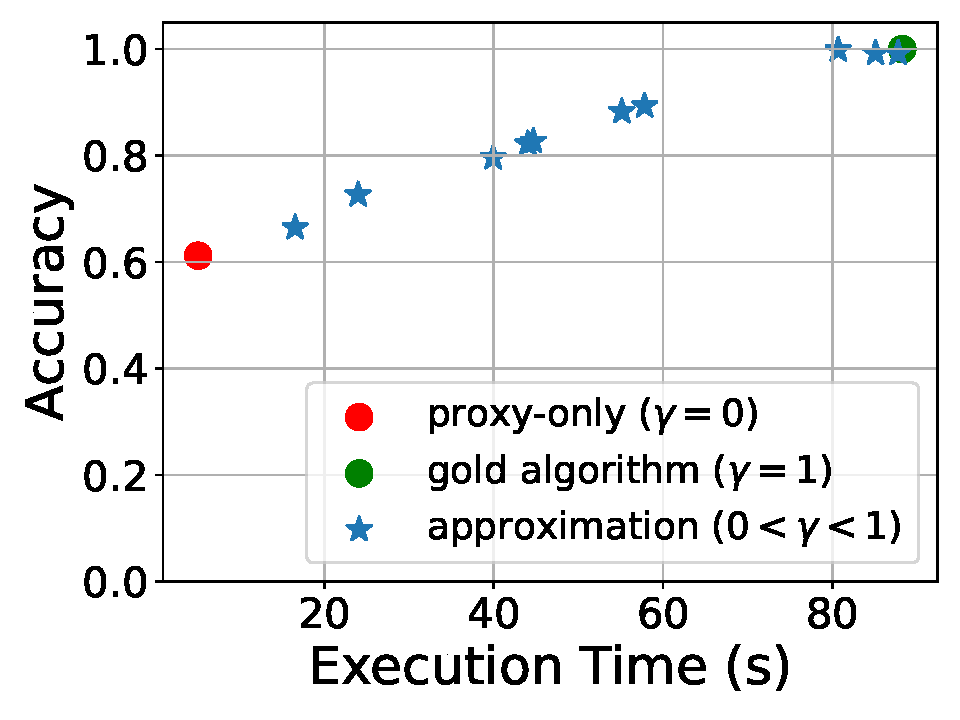
\includegraphics[width=0.5\linewidth]{figures/group_by.pdf}  
  \vspace{-.3cm}
   \caption{\small Classification accuracy vs. execution time (s) for the \sys sem\_group\_by over the ArXiv dataset. We compare the performance of implementing classifying each paper using the proxy only (red circle) or oracle only (green circle) to  our approximation with varied accuracy targets, at $\delta=0.2$ (stars).}
  \label{fig:groupby_cascades}
\vspace{-.3cm}
\end{figure}

Turning to the classification sub-task, we compare the performance of the gold algorithm to our approximation, which uses an embedding-based proxy here. Figure~\ref{fig:groupby_cascades} compares the execution time and classification accuracy of the oracle-based gold algorithm (green circle), our approximations using both the Llama-70B oracle LLM and embedding-based proxy at varied accuracy targets (blue stars), and the embedding-based proxy alone (red circle). We see that the proxy-only baseline is $17.4\times$ faster than the oracle, but about $39\%$ less accurate. Our approximation algorithm allows users to declaratively interpolate between these two extremes by varying the accuracy target. We also note that the sampling-based optimization procedure used to perform this optimization took less than 5 seconds, representing a small relative cost.


\begin{figure*}[t]
    \centering

    % Legend spanning the top row
    
\includegraphics[width=0.6\linewidth]{figures/ablation_legend.png}
    % \vspace{0.5cm}

    % Subfigures in a single row
    \begin{subfigure}[t]{0.2\linewidth}
        \centering
        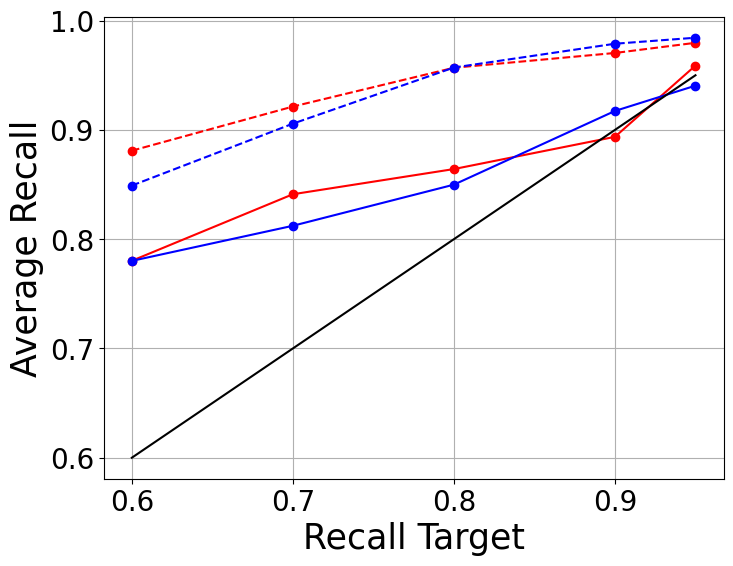
\includegraphics[width=\linewidth]{figures/recall_ablation.png}
        \caption{\small Observed vs Target Recall}
        \label{fig:recall_ablation}
    \end{subfigure}
    \hfill
    \begin{subfigure}[t]{0.2\linewidth}
        \centering
        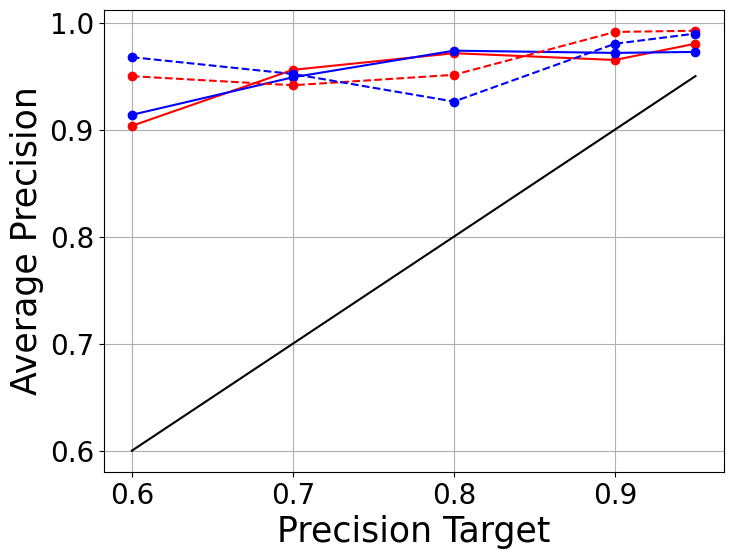
\includegraphics[width=\linewidth]{figures/precision_ablation.png}
        \caption{\small Observed vs Target Precision}
        \label{fig:precision_ablation}
    \end{subfigure}
    \hfill
    \begin{subfigure}[t]{0.2\linewidth}
        \centering
        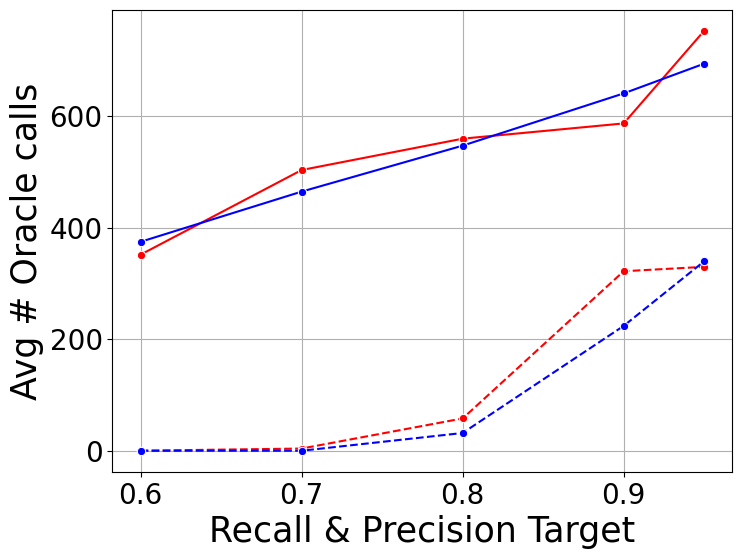
\includegraphics[width=\linewidth]{figures/numcall_ablation.png}
        \caption{\small \# Oracle Calls vs Accuracy Target}
        \label{fig:numcall_ablation}
    \end{subfigure}
    \hfill
    \begin{subfigure}[t]{0.2\linewidth}
        \centering
        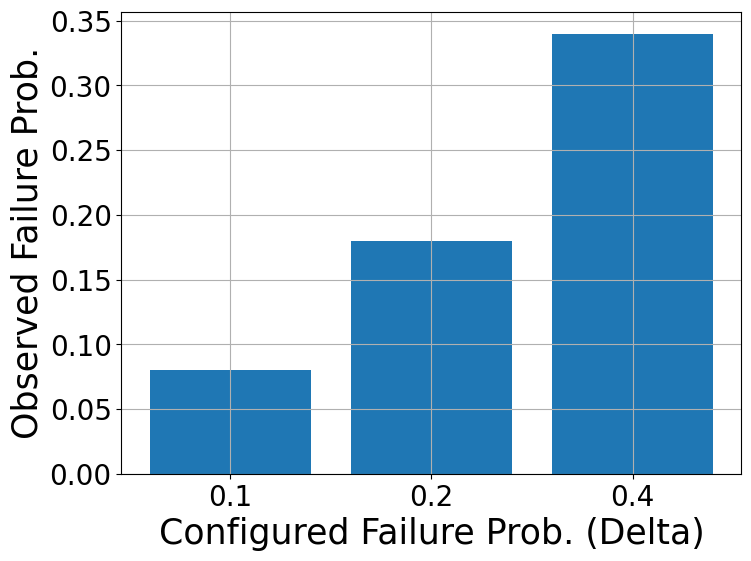
\includegraphics[width=\linewidth]{figures/failure_ablation.png}
        \caption{\small Observed vs Configured Failure Probability}
        \label{fig:delta_ablation}
    \end{subfigure}
    \vspace{-.3cm}
    \caption{\small We evaluate statistical accuracy guarantees with our semantic filter for fact-checking on the FEVER dataset. We show (a) average observed recall vs. configured recall targets ($\gamma_R)$, (b) average observed precision vs. configured precision targets ($\gamma_P)$, and (c) the number of oracle LLM calls vs. configured accuracy targets ($\gamma_R=\gamma_P$), using a Llama-70B oracle and either a Llama-8B proxy (dashed lines) or a weaker TinyLlama proxy (solid lines), for two different failure probabilities ($\delta=0.2, 0.4)$. We also show observed vs. configured failure probabilities using the TinyLlama proxy and Llama-70B oracle, for accuracy targets $\gamma_R = \gamma_P =0.9$.}
        \vspace{-.5cm}
    \label{fig:legend_and_subfigures}
\end{figure*}







\subsection{Accuracy Guarantees Evaluation}
\label{subsec:ablation}
Our approximation methods are designed to adaptively learn when to leverage a proxy to provide an accuracy guarantee, despite variations in proxy accuracy. To demonstrate the accuracy guarantees provided by our semantic operator optimizations, we study the \verb|sem_filter| performance on the fact-checking performance with varied proxy models, recall and precision targets and failure probability parameters. Figure~\ref{fig:recall_ablation} and Figure~\ref{fig:precision_ablation} demonstrate the average accuracy observed over 20 trials for varied recall targets and precision targets. We evaluate the filter approximation with both the Llama-8B proxy (solid lines) and a weaker proxy, with TinyLlama-1B (dashed lines) with a failure probability of $\delta=0.2$ (red) and $\delta=0.4$ (blue). As expected, the average recall and precision values increase with increasing accuracy targets for either metric. Figure~\ref{fig:numcall_ablation} demonstrates that decreasing the recall and precision target tends reduce the number of calls routed to the oracle. As expected, at a fixed accuracy target, our approximation requires more oracle calls when using the weaker proxy, in this case TinyLlama. Finally, in Figure~\ref{fig:delta_ablation} we record the percentage of 50 trials that do not meet the recall and precision target, both set to 0.9, using the TinyLlama proxy. The results confirm that the observed failure probabilities increase with the user-configured delta values, and are lower than the configured failure probabilities, as expected due to our conservative implementation.

